%%%%%%%%%%%%%%%%%%%%%%%%%%%%%%%%%%%%%%%%%%%%%%%%%%%%%%%%%%%%%%%%%
%%% %
%%% % weiiszablon.tex
%%% % The Faculty of Electrical and Computer Engineering
%%% % Rzeszow University Of Technology diploma thesis Template
%%% % Szablon pracy dyplomowej Wydziału Elektrotechniki 
%%% % i Informatyki PRz
%%% % June, 2015
%%%%%%%%%%%%%%%%%%%%%%%%%%%%%%%%%%%%%%%%%%%%%%%%%%%%%%%%%%%%%%%%%

\documentclass[12pt,twoside]{article}

\usepackage{weiiszablon}

\author{Rafał Stępień}

\studentID{EF-169625}

\title{Książkowy dziennik w chmurze}
\titleEN{Cloud-based book journal}

\newcommand{\rodzajPracyNo}{1}


\supervisor{dr inż. Mariusz Mączka}

\supervisorEN{Dr. Eng. Mariusz Mączka}

\abstract{Treść streszczenia po polsku}
\abstractEN{Treść streszczenia po angielsku}

\begin{document}

\maketitle

\blankpage

\tableofcontents

\clearpage
\blankpage

\section{Wstęp}
W dobie rosnącej cyfryzacji i dynamicznego rozwoju technologii mobilnych, coraz więcej osób poszukuje
nowoczesnych narzędzi wspierających codzienne czynności, w tym także zarządzanie swoimi pasjami i 
zainteresowaniami. Jedną z takich pasji, cieszącą się niezmienną popularnością, jest czytanie książek.
Wraz z rosnącą liczbą dostępnych tytułów zarządzanie osobistą biblioteką może stać się problematyczne.

Niniejsza praca dotyczy zaprojektowania i implementacji aplikacji mobilnej o nazwie 
„BookTracker”, stworzonej z wykorzystaniem technologii Jetpack Compose 
oraz zintegrowanej z internetową bazą danych Supabase. Aplikacja oferuje użytkownikom możliwość 
oznaczania książek jako posiadanych lub przeczytanych, śledzenia nadchodzących premier 
literackich oraz zarządzania osobistą biblioteką w sposób przejrzysty i dostępny z każdego 
miejsca, dzięki wykorzystaniu technologii chmurowych. Tematyka ta została wybrana ze względu 
na rosnącą popularność aplikacji wspierających organizację życia codziennego oraz potrzebę 
zapewnienia użytkownikom narzędzi umożliwiających wygodne i efektywne zarządzanie ich kolekcjami 
literackimi.

Zakres pracy obejmuje zaprojektowanie kluczowych funkcji aplikacji, implementację interfejsu 
użytkownika oraz integrację z bazą danych w chmurze. Głównym celem pracy jest stworzenie aplikacji mobilnej, 
która w przejrzysty sposób umożliwi użytkownikom zarządzanie osobistą biblioteką książek z 
wykorzystaniem technologii chmurowych.

\clearpage

\section{Podobne aplikacje}

W dzisiejszych czasach niemal każda aplikacja ma już swoje odpowiedniki na rynku. Podczas 
tworzenia aplikacji postawiono więc na skupienie się na grupie docelowej użytkowników, którzy
oczekują konkretnych rozwiązań.

\subsection{Bookmory}

Bookmory to przykład wielu istniejących aplikacji dzięki którym można zarządzać swoją biblioteką, do jej
odpowiedników można zaliczyć jeszcze kilka aplikacji takich jak: StoryGraph, Bookshelf, czy Bookly.
Każda z wymienionych aplikacji spełnia podobne zadania, a dla większości użytkowników wybór pomiędzy nimi
nie ma większego znaczenia, ponieważ różnice między nimi są minimalne.

Istnienie tych aplikacji zainspirowało stworzenie alternatywy, która będzie różniła się od swoich
poprzedników unikalną funkcjonalnością i skupieniem się na konkretnej grupie odbiorców.

\subsection{TV Time}

TV Time to popularna aplikacja służąca do śledzenia postępu oglądania seriali i filmów. 
Pomimo tego, że aplikacja ta nie ma możliwości zarządzania książkami i skupia się wyłącznie na 
produkcjach filmowych, to funkcjonalność śledzenia seriali stała się inspiracją do stworzenia
alternatywnej aplikacji do śledzenia postępu czytania książek. Główną różnicą do 
istniejących już rozwiązań jest skupienie się na seriach książek wydawanych w tomach i ułatwieniu
użytkownikom obserwowania i zarządzania książkami, które są ze sobą powiązane.

\clearpage

\section{Środowiska i technologie}

Wybór odpowiednich środowisk i technologii jest kluczowym elementem każdego projektu informatycznego, 
ponieważ wpływa zarówno na efektywność pracy, jak i na jakość końcowego rozwiązania. Ważnym jest 
przedstawienie wybranych rozwiązań i uzasadnienie dlaczego były one wybrane zamiast alternatywnych
opcji.

\subsection{Android Studio}

Android Studio to oficjalne zintegrowane środowisko programistyczne (IDE) do tworzenia aplikacji na system
Android bazujące na IntelliJ IDEA firmy JetBrains, stworzone i rozwijane przez firmę Google. Jest to 
kompleksowe narzędzie, które oferuje zestaw funkcji, mających na celu ułatwienie tworzenia, debugowania i
publikowania aplikacji.

Środowisko to jest nieustannie aktualizowane przez Google, aby wspierać najnowsze wersje systemu Android
oraz dodawać nowe funkcje. Android Studio obsługuje programowanie w językach takich jak Java, Kotlin 
(rekomendowany przez Google), a także w mniejszym stopniu w C++.

Kluczowym elementem jest edytor kodu, który obsługuje autouzupełnianie, refaktoryzację oraz podpowiedzi 
kontekstowe, co znacząco ułatwia pisanie czystego i efektywnego kodu.

Android Studio zostało wybrane ze względu na to, że jest najpełniejszym narzędziem do tworzenia aplikacji
na system android i w przeciwieństwie do np. Visual Studio Code, można praktycznie od razu rozpocząć
pracę zamiast zajmowania się instalowaniem rozszerzeń i potrzebnych komponentów. Android Studio oferuje 
wszystkie niezbędne funkcje w jednym pakiecie.

\subsection{Kotlin}

Kotlin to nowoczesny, statycznie typowany język programowania, który został stworzony przez firmę 
JetBrains i jest oficjalnie wspierany przez Google do tworzenia natywnych aplikacji na system Android. 
Kotlin jest zaprojektowany z myślą o prostocie, bezpieczeństwie i interoperacyjności z Javą - język ten 
jest w pełni kompatybilny z istniejącym ekosystemem Javy, co umożliwia łatwą integrację z istniejącym kodem i 
bibliotekami.

\subsection{Jetpack Compose}

Jetpack Compose to nowoczesny framework interfejsu użytkownika stworzony przez Google, który pozwala 
na tworzenie aplikacji na Androida w sposób deklaratywny. Zamiast używać tradycyjnych plików XML do 
definiowania widoków, Jetpack Compose umożliwia definiowanie interfejsu w kodzie Kotlin, co prowadzi 
do tworzenia prostszych, bardziej zwięzłych i łatwiejszych w utrzymaniu aplikacji.

Jetpack Compose został wybrany, ponieważ jest rozwiązaniem w pełni zintegrowanym z Androidem, 
co zapewnia najlepszą optymalizację i wydajność w tworzeniu aplikacji natywnych na tę platformę.

\subsection{Supabase}

Supabase to nowoczesna platforma typu Backend-as-a-Service (backend jako usługa), która umożliwia tworzenie
aplikacji z wykorzystaniem bazy danych PostgreSQL. Jest to narzędzie do budowy aplikacji, bez potrzeby 
zarządzania infrastrukturą serwerową.

Kluczowym elementem Supabase jest integracja z PostgreSQL, która umożliwia dostęp do bazy danych, oferującej
funkcje takie jak zaawansowane zapytania SQL, funkcje typu trigger oraz bezpieczeństwo na poziomie wiersza (RLS).
Supabase automatycznie tworzy RESTful API na podstawie tabel w bazie danych, co pozwala na szybkie
wdrażanie aplikacji. 

\subsection{GitHub}

GitHub to powszechnie używana platforma do zarządzania kodem źródłowym i współpracy w zespołach programistycznych, 
oparta na systemie kontroli wersji Git. Umożliwia śledzenie zmian w kodzie, zarządzanie historią projektu oraz
łatwą współpracę wielu programistów nad jednym projektem.

\clearpage

\section{Struktura bazy danych Supabase}



\begin{figure}[ht]
	\centering
	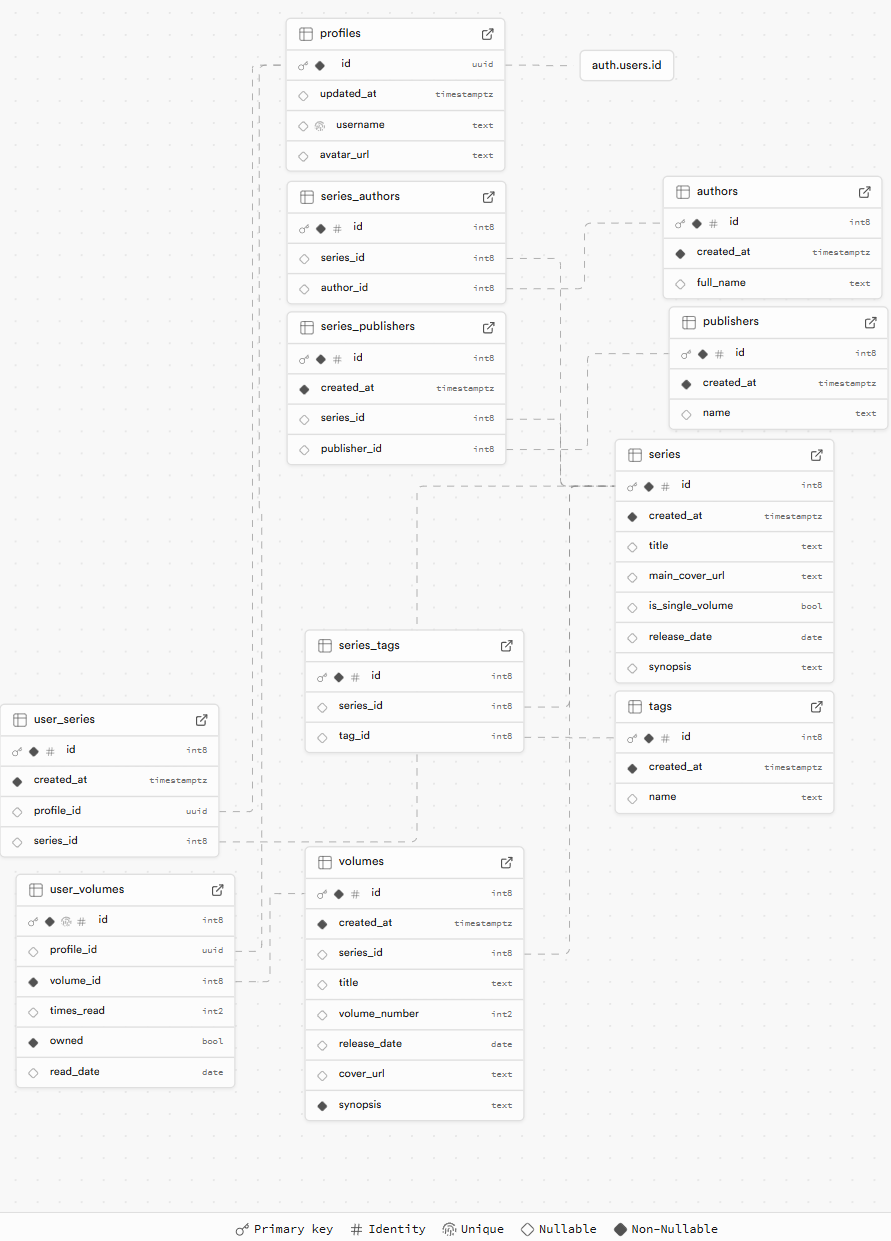
\includegraphics[width=1\textwidth]{figures/schemat1.png}
	\caption{Schemat bazy danych}
\label{Fig:schemat}
\end{figure}

\clearpage

\section{Architektura i struktura aplikacji}

Architektura aplikacji została oparta na wzorcu MVVM, co pozwala na efektywne zarządzanie stanem i separację 
logiki biznesowej od interfejsu użytkownika. Właściwa organizacja plików w projekcie jest kluczowa dla 
utrzymania porządku i skalowalności aplikacji, umożliwiając łatwe zarządzanie komponentami i ich zależnościami. 

\subsection{MVVM (Model-View-ViewModel)}

Model-View-ViewModel to popularny wzorzec architektoniczny stosowany w tworzeniu aplikacji, który pomaga w 
organizacji kodu i rozdzieleniu odpowiedzialności pomiędzy różne warstwy aplikacji. Jego głównym celem
jest zwiększenie modularności, łatwości testowania oraz oddzielenie logiki biznesowej od interfejsu użytkownika.

\begin{enumerate}[label=\alph*), leftmargin=1.25cm]
	\item Model reprezentuje warstwwę danych i logiki biznesowej. Jest odpowiedzialny za zarządzanie danymi,
	które mogą pochodzić z różnych źródeł, takich jak bazy danych, API czy pliki lokalne. Model nie zawiera
	żadnej logiki związanej z interfejsem użytkownika ani sposobem prezentacji danych,
	\item View (Widok) odpoawiada za warstwę prezentacji. Widok to interfejs użytkownika (UI), który jest
	odpowiedzialny za wyświetlenie danych i odbieranie interakcji od użytkownika. Widok powinien jedynie
	reagować na dane dostarczane przez ViewModel. W android widokiem są komponenty Jetpack Compose,
	\item ViewModel to warstwa pomiędzy modelem a widokiem. pobiera dane z modelu i przekształca je
	w taki sposób, aby były gotowe do wyświetlenia w widoku. Ponadto zarządza stanem widoku (np. przechowywaniem
	stanu aplikacji w przypadku zmiany orientacji ekranu).
\end{enumerate}

\subsubsection{Model}

W poniższym listingu 

\subsection{Struktura projektu}

\clearpage


\section{Tekst zasadniczy -- II}

{\subsubsection{Listingi programów}}

W pracy dyplomowej możesz umieszczać fragmenty programów. Pamiętaj, aby umieszczać krótkie, tylko najważniejsze fragmenty kodów źródłowych. Zawsze je komentuj w treści
pracy dyplomowej. Typowo w \LaTeX\ kody źródłowe umieszczane są w środowisku verbatim (\verb|\begin{verbatim}...\end{verbatim}|). Obecnie instnieje jednak bardziej nowoczesne i bardziej funkcjonalne środowisko \verb|lstlisting| (wymaga zainstalowanego w systemie pakietu \verb|listings|). Zwróć uwagę, że możesz kolorować składnię
automatycznie za pomocą parametru \verb|language|. W niniejszym dokumencie przedstawiono dwa przykłady listingów, Listing \ref{KodMatlab1} to przykład kodu źródłowego Matlaba, a poniżej Listing \ref{KodPerl1} dla Perl'a.\\
%\komentarz{

\begin{lstlisting}[language=Matlab,caption=Listing programu Matlab,label={KodMatlab1}]
i = 1
p = 3
for i = 1:10
    if i > 3
        i=i+p
    else 
        i=i+1
    end
end
\end{lstlisting}

\begin{lstlisting}[language=Perl,caption=Listing programu Perl,label={KodPerl1}]
  my $url ='http://pei.prz.edu.pl';
  use LWP::Simple;
  my $content = get $url;
  die "Couldn't get $url" unless defined $content;
  print $content;
  print "\n";
  print "Length " + length($content)
\end{lstlisting}

Z pewnością przeglądając źródło tego dokumentu zobaczysz, że kody źródłowe powinny mieć zdefiniowane parametry \verb|label|, aby łatwo w tekście do nich się odwoływać.
Numeracja linii jest w stylu domyślnie włączona (to przydatne, bo w treści pracy łatwo odwołać się dzięki temu do konkretnego wiersza w kodzie źródłowym), możesz je wyłączyć podając jako parametr \verb|numbers=none|. Więcej szczegółów możesz odnaleźć w sekcji \verb|\lstset| pliku arkusza styli. 
%}


\subsubsection{Numerowanie i punktowanie}

\begin{enumerate}[label=\arabic*), leftmargin=1.25cm]
	\item Pierwszy poziom (stosuje się numerowanie lub punktowanie). Formatowanie:
	akapit wyjustowany, wcięcie od lewej 0,75 cm, wysunięcie co 0,5 cm.
	\item Znakiem numerowania jest liczba (z kropką lub nawiasem).
		\begin{itemize}[label=-,labelsep=0.4cm,leftmargin=0.6cm]
			\item drugi poziom (stosuje się wyłącznie punktowanie). Formatowanie: akapit
			wyjustowany, wcięcie od lewej 1,25 cm, wysunięcie co 0,5 cm,
			\item znakiem punktowania jest łącznik lub mała litera alfabetu (z nawiasem). Nie
			zaleca się stosowania kropek, strzałek itp.,
			\item punktowane akapity rozpoczyna się minuskułą (małą literą), na końcu akapitu
			stawia się przecinek, ostatni punktowany akapit kończy się kropką.
		\end{itemize}
	\item Numerowane akapity rozpoczyna się majuskułą (wielką literą) i kończy kropką.
	\item Należy zwrócić uwagę, aby nie rozdzielać numerowania/punktowania pomiędzy
	kolejnymi stronami tekstu.
\end{enumerate}


\subsection{Wykaz literatury}

W wykazie literatury zamieszcza się wyłącznie pozycje, na które powołano się
w pracy. Kolejność numerów w wykazie – zgodna z kolejnością pojawiania się danej
pozycji w tekście.

Format akapitu: akapit wyjustowany, wysunięcie 0,75 cm. Prawidłowo opracowany
wykaz został zaprezentowany w niniejszym dokumencie w odpowiednim rozdziale, oznaczonym jako „Literatura”  (pozycja nr \cite{str} to zasoby internetowe,
\cite{Jakubczyk1997} – książka, \cite{Barski2011} – artykuł w czasopiśmie, \cite{dokum} – karta katalogowa).

{\subsection{Wydruk pracy}}

Przed wydrukiem należy usunąć ewentualne błędy literowe i sprawdzić prawidłową
interpunkcję. Przykładowo, łącznik zapisuje się za pomocą krótkiego minusa (np.
badawczo-rozwojowy) natomiast myślnik -- stosowany w zdaniach wtrąconych -- zapisuje
się za pomocą długiej pauzy. Dzielenie wyrazów według uznania Autora (można podzielić
długie wyrazy, powodujące duże „rozstrzelenie” tekstu w poprzedzającym wierszu. Zaleca się usunięcie pojedynczych znaków na końcu wiersza oraz podwójnych spacji w tekście.
Dla przedrostka „mikro” należy unikać stosowania litery „u” zamiast „$\mu$”. Znak „$\mu$” można
otrzymać przytrzymując lewy Alt i wpisując na klawiaturze numerycznej 0181 (podobnie
„stopień”: Alt-0176). W celu uniknięcia „rozstrzelenia” liczb i ich jednostek zaleca się
używanie „twardej” spacji pomiędzy liczbą i jednostką. Należy sprawdzić, czy tytuły
podrozdziałów/zakresów nie zostały jako pojedyncze wiersze na poprzedniej stronie oraz
czy rysunki/tabele i ich tytuły nie zostały rozdzielone pomiędzy kolejnymi stronami.

Pracę drukuje się dwustronnie. Zaleca się wydruk w kolorze. Przed wydrukiem
należy ponumerować strony (czcionka 10 pkt., dół strony, akapit wyśrodkowany). Strony
tytułowej oraz strony z podziękowaniem nie numeruje się. Spis treści rozpoczyna się od
strony numer 3 (lub 5, jeżeli zamieszczono podziękowania).

\clearpage

\section{Podsumowanie i wnioski końcowe}

1 $\div$ 3 stron merytorycznie podsumowanie najważniejszych elementów pracy oraz wnioski wynikające z osiągniętego celu pracy. Proponowane zalecenia i modyfikacje oraz rozwiązania będące wynikiem realizowanej pracy.

Ostatni akapit podsumowania musi zawierać wykaz własnej pracy dyplomanta i zaczynać się od sformułowania: „Autor za własny wkład pracy uważa: \ldots”.

\clearpage

\section*{Załączniki}
\addcontentsline{toc}{section}{Załączniki}

Według potrzeb zawarte i uporządkowane uzupełnienie pracy o dowolny materiał źródłowy (wydruk programu komputerowego, dokumentacja kons\-truk\-cyj\-no-\-tech\-no\-lo\-gicz\-na, konstrukcja modelu -- makiety -- urządzenia, instrukcja obsługi urządzenia lub stanowiska laboratoryjnego, zestawienie wyników pomiarów i obliczeń, informacyjne materiały katalogowe itp.).


\clearpage

\addcontentsline{toc}{section}{Literatura}

\begin{thebibliography}{4}
\bibitem{str} http://weii.portal.prz.edu.pl/pl/materialy-do-pobrania. Dostęp 5.01.2015.
\bibitem{Jakubczyk1997} Jakubczyk T., Klette A.: Pomiary w akustyce. WNT, Warszawa 1997.
\bibitem{Barski2011} Barski S.: Modele transmitancji. Elektronika praktyczna, nr 7/2011, str. 15-18.
\bibitem{dokum} Czujnik S200. Dokumentacja techniczno-ruchowa. Lumel, Zielona Góra, 2001.
\bibitem{Pawluk2001} Pawluk K.: Jak pisać teksty techniczne poprawnie, Wiadomości Elektrotechniczne, Nr 12, 2001, str. 513-515.
\end{thebibliography}

\clearpage

\makesummary

\end{document} 
